\section{Υπηρεσία εισαγωγής δεδομένων}

Το σύστημα εισαγωγής δεδομένων αρχικά ελέγχει τη βάση δεδομένων για την ύπαρξη δεδομένων ταινιών, συντελεστών, εταιριών και χωρών παραγωγής και ειδών ταινιών. Είναι σημαντικό για την συνέχεια να υπάρχουν δεδομένα σε όλες τις κατηγορίες. Αν δεν υπάρχουν δεδομένα σε οποιαδήποτε από όλες τις κατηγορίες προχωράει η άμεση εισαγωγή δεδομένων από άλλες υπηρεσίες. 

Το σύστημα εισαγωγής δεδομένων ανάλογα με τις ρυθμίσεις που του έχουν δοθεί θα προσπαθήσει να πάρει δεδομένα από διάφορες εξωτερικές υπηρεσίες και αφού τα συσχετίσει μεταξύ τους θα τα αποθηκεύσει στην βάση δεδομένων. 

Κατά την εκπόνηση της Πτυχιακής, παρουσιάστηκαν κάποια προβλήματα. Το κυριότερο ήταν η εύρεση μιας υπηρεσίας, η οποία να μπορεί να διαθέσει όλα τα δεδομένα που χρειάζονται για να λειτουργήσει σωστά η εφαρμογή. 

Μια από τις πιο διάσημες και αξιόπιστες υπηρεσίες η οποία διαθέτει API για εύκολη συλλογή δεδομένων είναι η TMDb (TheMovieDb) η οποία προσφέρει πλούσια στοιχεία για πάρα πολλές ταινίες. Δυστυχώς, αυτή η υπηρεσία είναι δημοφιλής μόνο στην προγραμματιστική κοινότητα και όχι ιδιαίτερα στο ευρύ κοινό με αποτέλεσμα να μη διαθέτει αξιόπιστες βαθμολογίες ταινιών καθώς υπάρχουν πολύ λίγες αξιολογήσεις. 

Από την άλλη η πιο διάσημη υπηρεσία δεδομένων ταινιών στο ευρύ κοινό είναι η IMDb (Internet Movie Database) η οποία όμως δεν διαθέτει υπηρεσία API για πρόσβαση στα δεδομένα. Διαθέτει όμως ένα μικρό κομμάτι των δεδομένων της σε μορφή συμπιεσμένου TSV για οικιακή ή μη-εμπορική χρήση. Μέσα σε αυτό το μικρό κομμάτι των δεδομένων που διαθέτει, υπάρχουν και βαθμολογίες ταινιών. 

Το άλλο πρόβλημα ήταν να βρεθεί ο τρόπος για να μπορούν να συσχετισθούν τα δεδομένα των βαθμολογιών ταινιών από την υπηρεσία IMDb με τα δεδομένα ταινιών από την υπηρεσία TMDb. Αυτό αντιμετωπίστηκε επιτυχώς
με την τελευταία ενημέρωση της υπηρεσίας TMDb με την οποία υπάρχει η δυνατότητα αναζήτησης ταινίας με το αναγνωριστικό κλειδί που προσφέρει η υπηρεσία IMDb.

Οι παραπάνω υπηρεσίες χρησιμοποιήθηκαν συνδυαστικά, πετυχαίνοντας την απόκτηση πλούσιων δεδομένων από την υπηρεσία TMDb και ταυτόχρονα πιο αξιόπιστων βαθμολογιών από την υπηρεσία IMDb.

\subsection{Βήμα 1ο - Δεδομένα από IMDb}
Με τις ρυθμίσεις που του
%ποιανού
δόθηκαν για αυτήν την πτυχιακή αρχικά παίρνει
%ποιός
ένα συμπιεσμένο αρχείο με δεδομένα βαθμολογιών ταινιών από το IMDb το αποσυμπιέζει και αποθηκεύει τα δεδομένα στην μνήμη. Η Μορφή
%Το περιεχόμενο?
δεδομένων του αρχείου είναι: το αναγνωριστικό μιας ταινίας η μιας σειράς (imdbId), η βαθμολογία της ταινίας/σειράς (rating) καθώς και το νούμερο των ψήφων με το οποίο βγήκε αυτή η βαθμολογία (voteCount). Έπειτα παίρνει ένα ακόμα συμπιεσμένο αρχείο από το IMDb του οποίου η μορφή
%..το οποίο περιέχει..
είναι το αναγνωριστικό μιας ταινίας η μιας σειράς (imdbId) και ο τύπος (titleType). Δηλαδή
%Ο τύπος διευκρινίζει εάν
αν είναι ταινία, σειρά ή κάτι άλλο. 

Αφού φορτώσει και τα 2 αρχεία στη μνήμη ξεχωρίζει τις εγγραφές που αναφέρουν μόνο ταινίες και μετά ξεχωρίζει τις εγγραφές οι οποίες έχουν αριθμό ψήφων μεγαλύτερο ή ίσο με μια σταθερά MINIMUM\_VOTES\_THRESHOLD και κρατάει τα 3 αρχικά πεδία του πρώτου αρχείου. Η Σταθερά αυτή για αυτό το σενάριο είναι 1000.
%σενάριο
%Η σταθερά αυτή έχει καθοριστεί ως 1000 ψήφοι.
%discard entry process
%σύνδεση με 2ο βήμα

\begin{figure}[h]
  \centering
  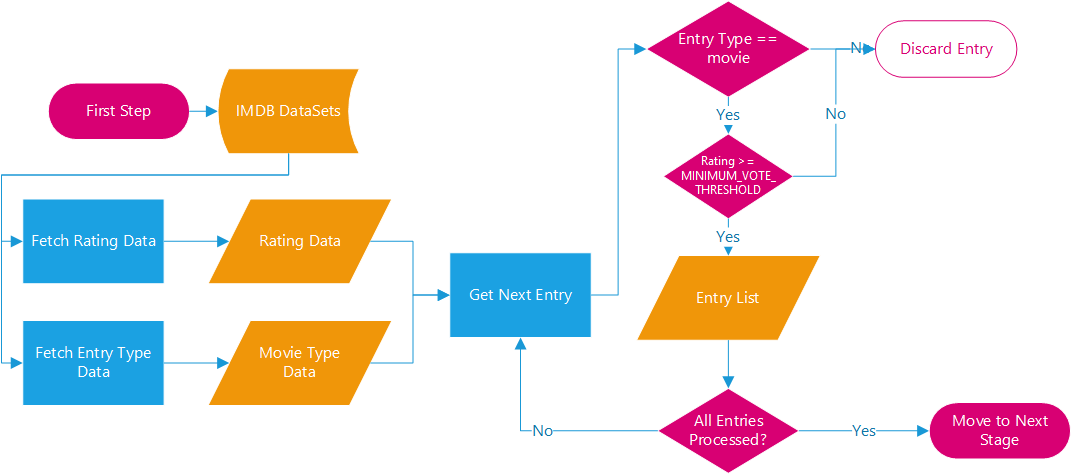
\includegraphics[width=150mm]{Chapters/5 - Architecture/Import/Images/imdb_flowchart.png}
  \caption{Διάγραμμα ροής δεδομένων από IMDB}
  \label{flowchart:imdbImport}
\end{figure}
\subsection{Βήμα 2ο - Δεδομένα από TMDb}
Στο 2ο βήμα αφού έχουμε τα δεδομένα που χρειάζονται από το πρώτο, δημιουργεί και προγραμματίζει για εκτέλεση ασύγχρονα ερωτήματα ζητώντας πλήρη δεδομένα ταινιών για κάθε αναγνωριστικό ταινίας που έχουμε στην υπηρεσία TMDb. 

Ο στόχος δεν είναι μόνο η απόκτηση δεδομένων ταινιών αλλά και συντελεστών, εταιριών και χωρών παραγωγής, και ειδών ταινιών, συνεπώς αφού πάρει τα δεδομένα ταινιών θα χρονοδρομολογήσει και άλλα ασύγχρονα ερωτήματα στην εν λόγω υπηρεσία για να πάρει και τα υπόλοιπα δεδομένα. 

Αφού τελειώσει αυτή η διαδικασία, συσχετίζει όλα τα δεδομένα μεταξύ τους και τα εισάγει στην βάση δεδομένων για περαιτέρω επεξεργασία από κάποιο άλλο σύστημα. 
\begin{figure}[h]
  \centering
  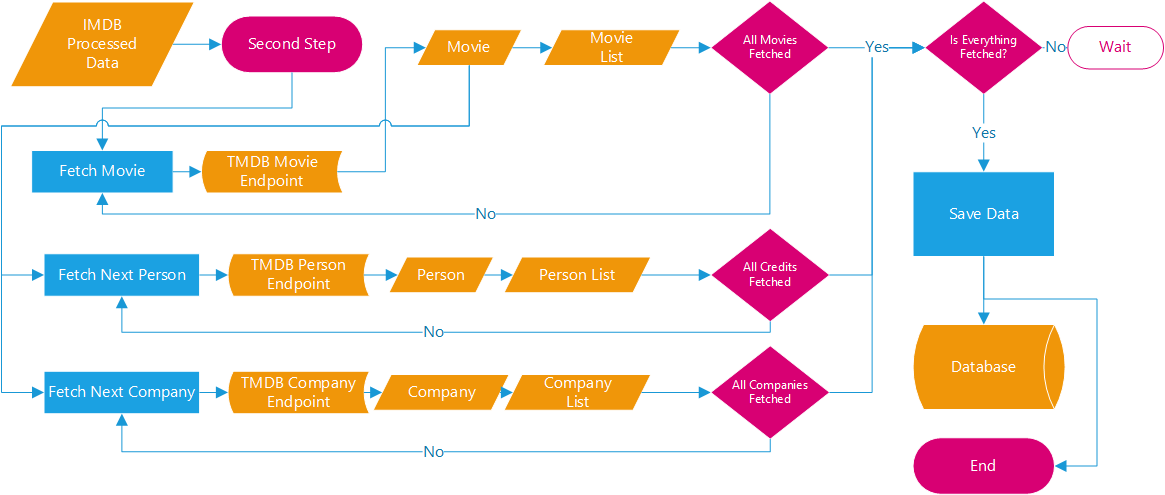
\includegraphics[width=150mm]{Chapters/5 - Architecture/Import/Images/tmdb_flowchart.png}
  \caption{Διάγραμμα ροής δεδομένων από TMDb}
  \label{flowchart:tmdbImport}
\end{figure}